\chapter{Théorie des Semi-conducteurs et des Solides}
%\section{Chapter Overview}
Dans ce chapitre, nous aborderons le concept de semi-conducteur. Nous décrirons le type de matériau que cela représente, basé sur le concept de bandes d'énergie. Sous forme solide, un semi-conducteur comme le silicium forme un cristal, donc une attention particulière est portée au comportement des électrons dans un cristal. Le nombre de porteurs de charge dans un semi-conducteur (qui peuvent être des électrons, comme dans un métal, ou des trous, qui n'existent pas dans un métal) est calculé. Pour augmenter le nombre de porteurs, nous dopons le semi-conducteur avec des impuretés. Ensuite, nous considérons les phénomènes de transport les plus importants dans les semi-conducteurs, à savoir la dérive et la diffusion. Enfin, nous discutons de la génération et de la recombinaison de paires électron-trou et établissons les équations de continuité.
\section{Les Semi-conducteurs}
Nous appelons semi-conducteurs les éléments de la quatrième colonne de la table périodique. Des exemples sont le carbone (C), le silicium (Si) et le germanium (Ge). Ces éléments ont 4 électrons sur leur couche externe et ont tendance à former 4 liaisons covalentes avec les atomes voisins pour obtenir une structure octet stable. En se liant, ils forment un motif régulier appelé cristal.\\
Le silicium, l'atome de semi-conducteur le plus couramment utilisé en électronique, a une couche externe ($n=3$) avec un orbitale $3s^2$ complètement rempli et un orbitale $3p^2$ partiellement rempli. Pour former des liaisons, les orbitales de la couche externe interagissent et subissent une hybridation $sp^3$. La conséquence est que les 4 liaisons covalentes sont uniformément espacées dans l'espace, formant des liaisons d'environ $109^{\circ}$ les unes avec les autres.\\
La partie gauche de la figure \ref{fig:crystal} montre une seule cellule de la structure cristalline du silicium. Les points bleus représentent un seul atome de silicium, avec des liaisons covalentes à $4$ atomes voisins. La figure de droite montre une représentation simplifiée en 2 dimensions du même cristal.\\
Parfois, un élément composé peut également être un semi-conducteur. L'arséniure de gallium (GaAs) est un composé composé d'atomes de gallium et d'arsenic. C'est un semi-conducteur composé III-V, ce qui signifie qu'il est composé d'éléments des groupes III et V de la table périodique.

\begin{figure}[htbp]
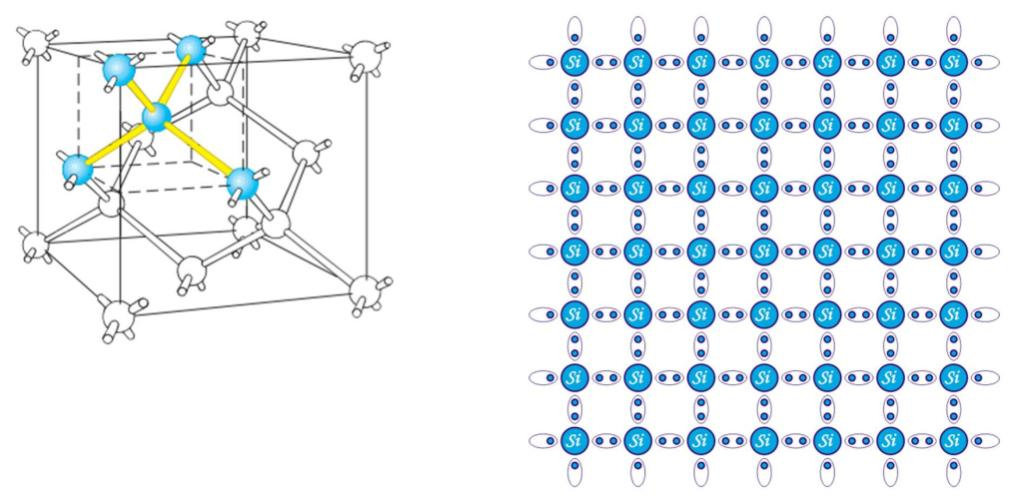
\includegraphics[width=12cm]{figures/ch01/crystal.jpg}
\caption{Silicon crystal (left) - schematic representation (right)}
\label{fig:crystal}
\end{figure} 

\subsection{Structure de bande}
Lorsque les atomes sont très éloignés, ils ne s'influencent pas mutuellement et nous pouvons trouver leur fonction d'onde $\Psi(x, t)$ en résolvant l'équation de Schrödinger pour un seul électron en orbite autour d'un noyau fixe. Cela résulte dans le spectre d'énergie discret bien connu associé à chaque fonction d'onde. Cependant, lorsque les atomes se rapprochent, leurs électrons dans la couche externe commencent à interagir les uns avec les autres. Selon le principe d'exclusion de Pauli, ils ne peuvent plus occuper les mêmes niveaux d'énergie.\\
Supposons que $N$ atomes de Si sont initialement très éloignés, et nous les rapprochons avec pour objectif de former un cristal. Nous avons donc $2N$ électrons au niveau d'énergie de l'orbitale $3s$, et $2N$ électrons dans l'orbitale $3p$, où il y a $6N$ niveaux disponibles. Lorsque les atomes sont suffisamment proches, ils interagissent et les niveaux d'énergie doivent légèrement descendre ou monter pour être conformes au principe d'exclusion de Pauli. Les niveaux sont toujours discrets, mais étant donné que $N$, le nombre d'atomes dans le cristal, est un nombre énorme ($N \approx 10^{20}$ atomes par cm$^3$), nous pouvons considérer la bande d'énergie résultante comme un spectre continu (voir la figure \ref{fig:bandstructure}). À partir d'un certain espacement de réseau, les bandes $3s$ et $3p$ fusionnent pour former une seule bande. Lorsque les atomes se rapprochent suffisamment pour former un cristal comme dans la figure \ref{fig:crystal}, nous observons que les bandes se séparent à nouveau. À la distance interatomique dans le réseau cristallin ($5.43 \AA$ pour le silicium), il y a une \emph{bande de valence} avec des énergies jusqu'à une énergie $E_V$ et une \emph{bande de conduction} avec des énergies supérieures à $E_C > E_V$. Entre les bandes se trouve une plage interdite où aucun électron ne peut exister. Cette plage est appelée \emph{gap} de bande et la différence entre $E_C$ et $E_V$ est l'\emph{énergie de gap} $E_g$.

\begin{figure}[h!]
\centering
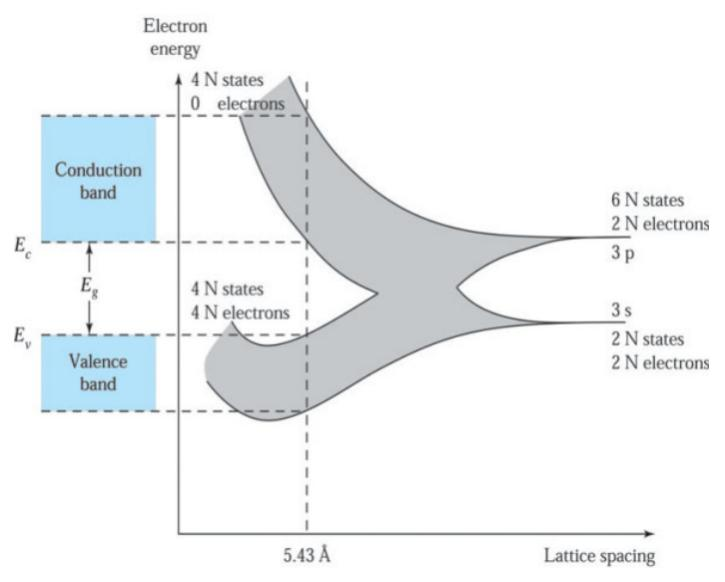
\includegraphics[width=12cm]{figures/ch01/bandstructure.jpg}
\caption{Band structure formation}
\label{fig:bandstructure}
\end{figure} 

\section{Électrons et trous}
À une température de $0$ K, tous les $4N$ électrons se trouvent dans la bande de valence. Cela signifie qu'ils font tous partie d'une liaison covalente entre deux atomes de silicium. Cependant, à mesure que la température augmente, les électrons obtiennent plus d'énergie thermique et certains d'entre eux peuvent rompre la liaison covalente et devenir des électrons libres qui peuvent se déplacer à travers le cristal. Ils ont acquis suffisamment d'énergie pour passer de la bande de valence à la bande de conduction. Lorsqu'une liaison covalente est rompue, l'électron laisse derrière lui une position vide. Cette position libre peut être occupée par un autre électron provenant d'une autre liaison électronique. Ce mécanisme est illustré sur la figure \ref{fig:breakingbond}. Une position vide dans une liaison est appelée un \emph{trou}. Puisque les électrons sautant d'un trou à l'autre font bouger le trou dans le cristal, nous pouvons considérer un trou comme une autre particule en mouvement, avec une charge positive $+q$.\\
Il existe également d'autres mécanismes en plus de l'agitation thermique qui peuvent fournir suffisamment d'énergie à un électron pour qu'il saute de la bande de valence à la bande de conduction, comme un photon qui frappe avec une énergie $E$ suffisamment élevée (donc une fréquence $\nu$, puisque $E = \hbar \nu$). Le fond de la bande de conduction $E_C$ correspond à l'énergie potentielle d'un électron, tout comme le sommet de la bande de valence $E_V$ correspond à l'énergie potentielle d'un trou.

\begin{figure}[h!]
\centering
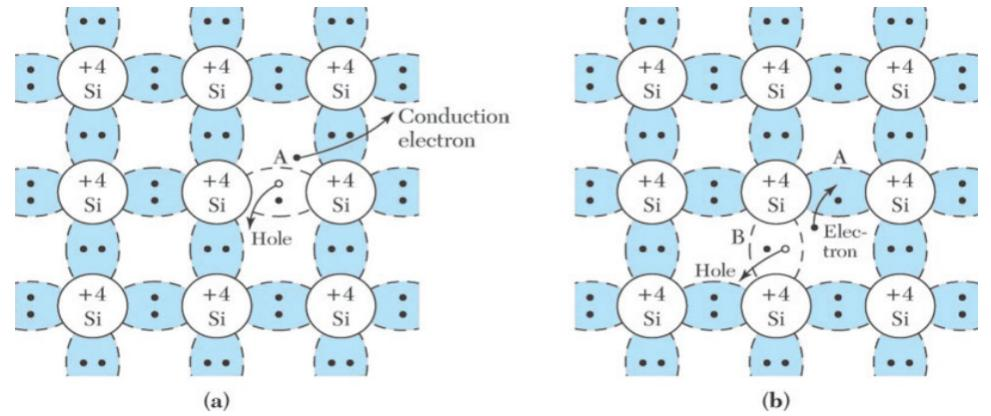
\includegraphics[width=12cm]{figures/ch01/breakingbond.jpg}
\label{fig:breakingbond}
\caption{Creation of electron hole pair by breaking of covalent bonds}
\end{figure} 

Lorsque l'on considère différentes directions dans le réseau cristallin, la structure de bande diffère car la distance interatomique dépend de la direction. La direction de propagation d'une fonction d'onde est déterminée par son vecteur d'onde $\vec{k}$, et $k$ est directement lié à l'impulsion $p$ par la relation :
$$\vec{p} = \hbar \vec{k}$$
C'est pourquoi ces \emph{diagrammes de bande} sont généralement tracés en fonction de l'énergie $E$ en fonction de l'impulsion $p$. La figure \ref{fig:indirectbandgap} montre les diagrammes de bande pour le silicium (à gauche) et le GaAs (à droite).\
Ces figures montrent que pour certains semi-conducteurs, comme le GaAs, le minimum de la bande de conduction se situe dans la même direction que le maximum de la bande de valence. Ces semi-conducteurs sont appelés semi-conducteurs à \emph{bande interdite directe}. D'autres, comme le silicium, ont des directions différentes pour ces deux points et sont donc appelés semi-conducteurs à \emph{bande interdite indirecte}.

\begin{figure}[h!]
\centering
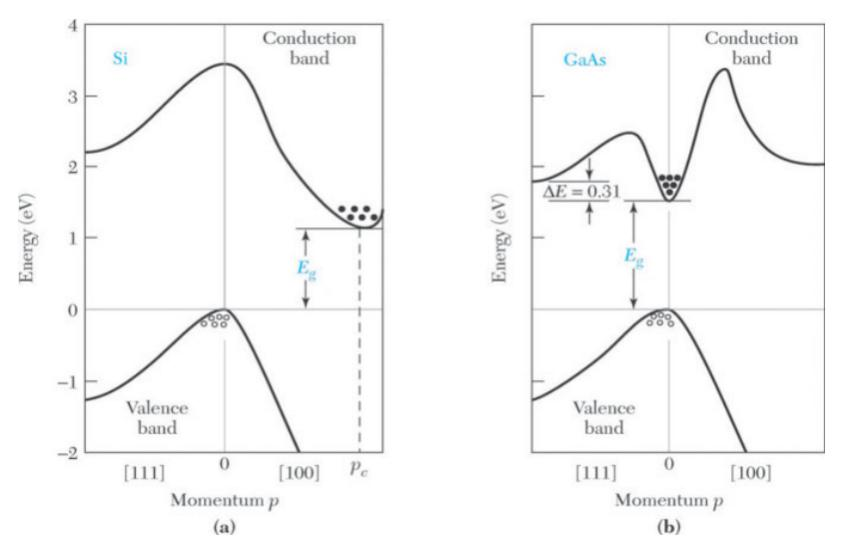
\includegraphics[width=12cm]{figures/ch01/indirectbandgap.jpg}
\caption{Band diagrams: (a) Si and (b) GaAs} 
\label{fig:indirectbandgap}
\end{figure} 

\subsection{Masse effective}
Un électron libre - non entravé par d'autres particules et leurs fonctions potentielles - a une masse $m_0 = 9,11 \; 10^{-31}$ kg. Cependant, dans un cristal, les électrons de la bande de conduction sont influencés par les noyaux et les autres électrons. Pour déterminer leur comportement, nous devrions résoudre l'équation de Schrödinger pour toutes ces particules. À la place, nous introduisons le concept de masse effective, qui peut être considérée comme la masse apparente d'une particule (électron ou trou) dans un cristal.\\
Chaque fonction d'onde a une vitesse de groupe $v_g = \frac{d \omega}{dk}$ et puisque $E = \hbar \omega$, nous avons $v_g = \frac{1}{\hbar}\frac{dE}{dk}$. Mais comme l'augmentation d'énergie $dE$ de la particule peut être considérée comme le résultat du travail $dW$ effectué par une force $F$ via la relation $dW = F dl = F v_g dt$ où $dl$ est le déplacement en temps $dt$, nous pouvons simplifier cette relation en $\frac{dk}{dt} = \frac{F}{\hbar}$.\\
Si une particule subit une variation de vitesse de groupe - une accélération $a$ - nous pouvons affirmer que:
\begin{equation} \label{eq1}
\begin{split}
a &= \frac{dv_g}{dt} = \frac{1}{\hbar}\frac{d}{dt}\frac{dW}{dk} \\
  &= \frac{1}{\hbar}\frac{d^2 W}{dk^2}\frac{dk}{dt} \\
  &= \frac{1}{\hbar^2}\frac{d^2 W}{dk^2}F
\end{split}
\end{equation}

Cela donne une relation entre la force appliquée $F$ et l'accélération résultante $a$. Ainsi, selon la deuxième loi de Newton $F = ma$, nous pouvons interpréter la constante de proportionnalité comme la masse effective de la particule:
$$
m^* = \hbar^2 \Big[\frac{d^2 W}{dk^2}\Big]^{-1}
$$
La masse effective d'un électron ou d'un trou est donc déterminée par la courbure locale de la relation $E-k$ dans le diagramme de bande. À partir de la figure \ref{fig:indirectbandgap}, nous voyons que pour le silicium, la courbure de la bande de conduction est plus élevée que celle de la bande de valence. Par conséquent, la masse effective $m_e^*$ d'un électron sera plus petite que celle d'un trou $m_h^*$.

\subsection{Nombre de porteurs}
Nous pouvons calculer la concentration d'électrons et de trous dans le silicium pur en utilisant la statistique quantique. La distribution des fermions (comme les électrons) est déterminée par la distribution de Fermi-Dirac :
$$
F(E) = \frac{1}{1-e^{(E-E_F)/kT}}
$$
qui donne la probabilité qu'à la température $T$, un électron occupe le niveau d'énergie $E$. $E_F$ est le niveau de Fermi, un niveau de référence où la probabilité d'occupation est exactement de moitié, et $k$ est la constante de Boltzmann (à ne pas confondre avec le nombre d'onde $k$).\\
Nous considérons également le nombre d'états autorisés à un niveau d'énergie $E$. Nous savons déjà que entre $E_V$ et $E_C$, aucun état n'est disponible car c'est la région de la bande interdite. Pour respectivement les électrons dans la bande de conduction et les trous dans la bande de valence, nous avons que :
\begin{equation} 
\begin{split}
N_C(E)  &= \frac{4 \pi}{\hbar} (2 m_e^*)^{3/2} (E - E_C)^{1/2} \\
N_V(E)  &= \frac{4 \pi}{\hbar} (2 m_h^*)^{3/2} (E_V - E)^{1/2}
\end{split}
\end{equation}
où $N_C(E)$ et $N_V(E)$ représentent la densité d'états par unité de volume dans la bande de conduction et la bande de valence.\
Pour calculer la densité de porteurs, nous multiplions la densité d'états par la probabilité qu'un état soit occupé, et intégrons sur les niveaux d'énergie pertinents. Nous notons $n$ pour le nombre d'électrons dans la bande de conduction, et $p$ pour le nombre de trous dans la bande de valence :
\begin{equation}
	\begin{split}
		n = \int_{E_C}^{\infty} N_C(E) F_e(E) dE\\
		p = \int_{-\infty}^{E_V} N_V(E) F_h(E) dE
		\label{eq:carrier_density}
	\end{split}
\end{equation}
Puisque $E_C$ et $E_V$ sont tous deux suffisamment éloignés du niveau de Fermi, nous pouvons simplifier la distribution de Fermi-Dirac et obtenir une distribution de Boltzmann standard :
\begin{equation} 
\begin{split}
F_e(E) \approx e^{-(E-E_F)/kT}\text{ if }E-E_F \gg kT \\
F_h(E) \approx e^{(E-E_F)/kT}\text{ if }E-E_F \ll kT 
\label{eq:boltzmann_simple}
\end{split}
\end{equation}
En substituant \ref{eq:boltzmann_simple} dans \ref{eq:carrier_density}, on obtient :
\begin{equation} 
\begin{split}
n = N_C \; e^{-(E_C-E_F)/kT} \text{ with } N_C = \ldots\\
p = N_V \; e^{-(E_F-E_V)/kT} \text{ with } N_V = \ldots
\label{eq:carrier_density2}
\end{split}
\end{equation}

La figure \ref{fig:carrierdensity} représente le schéma de bande, la densité d'états $N(E)$, la distribution des porteurs $F(E)$ et les résultats finaux.

\begin{figure}[h!]
\centering
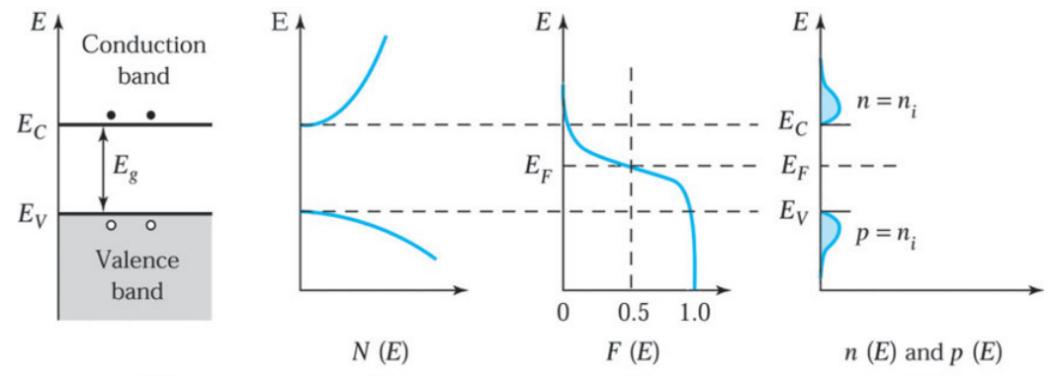
\includegraphics[width=12cm]{figures/ch01/carrierdensity.jpg}
\caption{Carrier density} 
\label{fig:carrierdensity}
\end{figure} 


Dans le silicium pur, chaque électron dans la bande de conduction donne naissance à un trou dans la bande de valence - d'où $n = p$ et $E_F$ se situe presque à mi-chemin entre $E_V$ et $E_C$ (la petite différence est due à une différence de masse effective entre les trous et les électrons). On dit que $n = p = n_i$, la densité de porteurs intrinsèques. En général, à température ambiante, $n \approx 10^{10}/cm^3$. Si nous multiplions les équations pour $n$ et $p$, le niveau de Fermi disparaît :
\begin{equation}
n p = n_i^2 = N_C \; e^{-(E_C-E_F)/kT} \; N_V \; e^{-(E_F-E_V)/kT} = N_C N_V \; e^{-E_g/kT}
\label{eq:np}
\end{equation}
\section{Impuretés donneuses et accepteuses}
La densité de porteurs intrinsèques $n_i$ est assez faible, et le silicium pur est un mauvais conducteur. Cependant, nous pouvons augmenter le nombre de porteurs (soit des trous, soit des électrons) avec un processus appelé \emph{dopage}. Le dopage consiste à remplacer certains des atomes de silicium par des atomes du groupe III (atomes accepteurs) ou du groupe V (atomes donneurs) du tableau périodique. Si les atomes de remplacement sont des atomes donneurs (comme l'arsenic ou le phosphore), ils se lient aux atomes de silicium voisins mais ont toujours un électron supplémentaire. Cet électron n'est que faiblement lié au noyau et peut facilement passer à la bande de conduction - sans créer de trou. De même, les atomes du groupe III, comme le bore, ont un électron en moins pour créer $4$ liaisons covalentes. Cependant, s'ils peuvent arracher un électron à une autre liaison, ils peuvent l'utiliser pour obtenir une structure octet et en même temps ont créé un trou. Les deux processus sont schématiquement représentés sur la figure \ref{fig:doping}. Le dopage élimine également la dépendance de la concentration de porteurs majoritaires par rapport à la température.

\begin{figure}[h!]
\centering
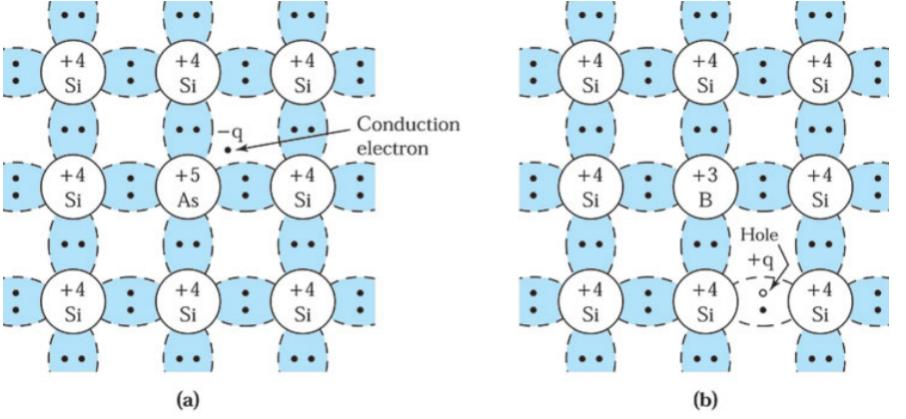
\includegraphics[width=12cm]{figures/ch01/doping.jpg}
\caption{Doping with (a) donor atoms and (b) acceptor atoms} 
\label{fig:doping}
\end{figure} 

Conventionnellement, nous utilisons $N_d$ pour la concentration de donneurs et $N_a$ pour la densité d'accepteurs. Ils ont des valeurs typiques de $10^{16}/cm^3$. Cela est beaucoup plus faible que le nombre d'atomes ($\sim 10^{20}/cm^3$), mais beaucoup plus élevé que la concentration intrinsèque de porteurs $n_i$ ($\sim 10^{10}/cm^3$). Nous parlerons de semi-conducteurs de type n ou p lorsque nous parlons de dopage avec des donneurs ou des accepteurs, respectivement.\\
L'expression \ref{eq:carrier_density2} reste valable, également dans un semi-conducteur dopé. Par conséquent, les porteurs de charge majoritaires (électrons dans un semi-conducteur de type n, trous dans un semi-conducteur de type p) sont largement plus nombreux que les porteurs de charge minoritaires (trous dans un semi-conducteur de type n, électrons dans un semi-conducteur de type p). Dans le cas d'un semi-conducteur de type n, par exemple, nous supposons que tous les atomes donneurs perdent leur électron supplémentaire et deviennent ionisés. Ainsi, $n_n = N_d \approx 10^{16}/cm^3$. En conséquence, $p_n = n_i^2/n_n \approx 10^{4}/cm^3$. Notez le sous-script $n$ pour indiquer qu'il s'agit d'un semi-conducteur de type n.\\
Le niveau de Fermi pour les semi-conducteurs dopés (ou \emph{extrinsèques}) ne se situe plus à mi-chemin entre la bande de valence et la bande de conduction. Puisque:
$$
n_n = N_d =  N_C e^{-(E_C-E_{Fn})/kT}\Rightarrow E_{Fn} = E_C - kT \ln \frac{N_d}{N_C} \\
$$
et nous savons également que $E_{i} = E_C - kT \ln \frac{n_i}{N_C}$ pour un semi-conducteur intrinsèque. Ainsi:
$$
E_{Fn} = E_{i} + kT \ln \frac{N_d}{n_i}
$$
and 
$$
E_{Fp} = E_{i} - kT \ln \frac{N_a}{n_i}
$$
Cela signifie que dans un semi-conducteur de type n, le niveau de Fermi se situe au-dessus du niveau de Fermi intrinsèque, tandis que dans un semi-conducteur de type p, il se situe en dessous. De plus, le niveau de Fermi se rapproche de la bande de conduction (de valence) si $N_d$ ($N_a$) est plus élevé. La figure \ref{fig:doping2} montre comment la distribution de charges change dans un semi-conducteur de type n, en raison d'un déplacement du niveau de Fermi $E_{Fn}$. Notez également le surplus d'électrons par rapport aux trous, puisque presque tous les électrons de la bande de conduction proviennent de l'ionisation des atomes donneurs.
\begin{figure}[h!]
\centering
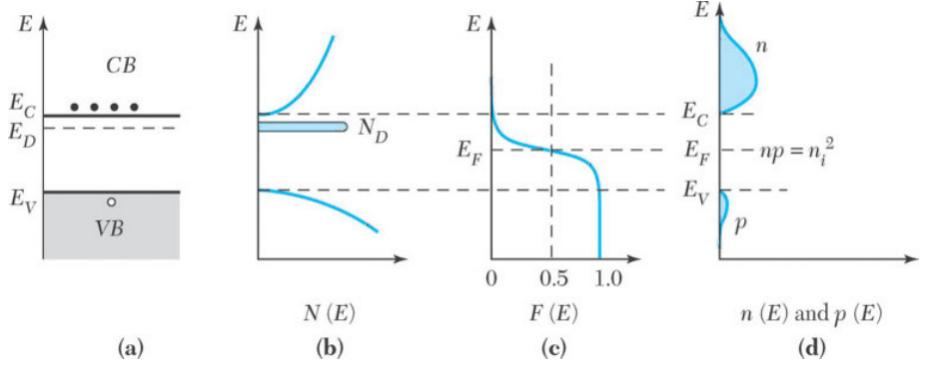
\includegraphics[width=13cm]{figures/ch01/doping2.jpg}
\caption{Carrier density due to donor doping in n-type semiconductor} 
\label{fig:doping2}
\end{figure}


Si nous transformons les énergies en potentiels via la relation $E = -q V$ et définissons $V$ comme la différence de potentiel entre le niveau de Fermi intrinsèque et réel : $V = V_{Fi} - V_F$, nous pouvons réécrire ces équations et obtenir les \emph{équations de Boltzmann}:
\begin{equation} 
\begin{split}
n &= n_i \; e^{qV/kT}  = n_i e^{V/v_{th}}  \\
p &= n_i \; e^{-qV/kT} = n_i e^{-V/v_{th}}
\label{eq:boltzamnn_eqns}
\end{split}
\end{equation}
avec $v_{th} = kT/q$ la tension thermique ($\approx 26$ mV à $T=300$ K). Ces équations ne sont valables qu'à l'équilibre thermique, c'est-à-dire lorsqu'il n'y a pas d'écoulement de charges.

\subsection{Transport de Porteurs}
Plusieurs mécanismes de transport de porteurs existent dans un semi-conducteur. Nous discutons ici les deux plus courants : le courant de dérive, dû à la présence d'un champ électrique, et le courant de diffusion, dû à un gradient de concentration.
\subsection{Courant de Dérive}
En l'absence d'un champ électrique, les charges se déplacent de manière aléatoire en raison de leur énergie thermique. Cependant, puisque le mouvement est aléatoire, il n'existe aucune direction préférentielle de déplacement. Cela change lorsque un champ électrique externe est appliqué. En présence d'un champ électrique $\mathcal{E}$, un électron avec une charge $-q$ est accéléré par une force $F_1 = -q \mathcal{E}$. Cependant, en même temps, la charge interagit avec le réseau cristallin et est ralentie par des collisions avec les atomes et les impuretés. Cette force d'amortissement $F_2$ est proportionnelle à la vitesse de la particule : $F_2 = -\alpha v_d$, avec $\alpha$ le facteur d'amortissement. Ainsi :
$$
m_e^* \frac{d v_d}{dt}  = -q \mathcal{E}  - \alpha v_d
$$
La particule atteindra une vitesse d'équilibre $v_{d0}$ lorsque $\frac{d v_d}{dt} = 0$, ainsi $v_{d0} = \frac{-qE}{\alpha}$. Nous pouvons résoudre l'équation du premier ordre pour une particule qui est initialement à une vitesse $v_d(0) = 0$ et obtenir $v_d(t) = v_{d0} e^{-t/ \tau_e}$ où $ \tau_e = \frac{m_e^*}{\alpha}$ est un temps caractéristique appelé \emph{temps de relaxation}. Il est proportionnel au temps nécessaire pour atteindre $v_{d0}$ et est de l'ordre de $1$ ps.\
D'un point de vue macroscopique, pour calculer le courant électronique total, nous devons faire la moyenne sur tous les électrons disponibles pour la conduction, c'est-à-dire les électrons présents dans la bande de conduction. Après quelques calculs, nous obtenons pour la densité de courant électronique $J_n = q \mu_n n \mathcal{E}$ avec la \emph{mobilité des électrons} $\mu_n = \frac{q \tau_e}{m_e^*}$. Une expression similaire peut être trouvée pour la densité de courant de trous $J_p$. Le courant total est la somme des deux:
\begin{equation}
    J = J_n + J_p = q(\mu_n n + \mu_p p) \mathcal{E} = \sigma \mathcal{E}
\end{equation}
Ceci est la formulation de la loi d'Ohm pour un semi-conducteur.
\subsection{Structure de bande sous polarisation}
Nous considérons la conduction dans un matériau semi-conducteur homogène due à un champ électrique. La figure \ref{fig:bandbiasing} montre un semi-conducteur de type n et son diagramme de bande à l'équilibre thermique (à gauche) et le diagramme de bande lorsqu'une tension de polarisation positive est appliquée à la borne de droite (à droite). Lorsqu'un champ électrique E est appliqué à un semi-conducteur, chaque électron subit une force $-q \mathcal{E}$ du champ. La force est égale au gradient négatif de l'énergie potentielle :
$$
-q \mathcal{E} = \frac{dE_C}{dx}
$$
Puisque nous nous intéressons au gradient de l'énergie potentielle, nous pouvons utiliser n'importe quelle partie du diagramme de bande qui est parallèle à $E_C$. Il est pratique d'utiliser le niveau de Fermi intrinsèque $E_{i}$ car nous l'utiliserons lorsque nous considérerons les jonctions p-n. Ainsi:
$$
\mathcal{E} = -\frac{1}{q}\frac{dE_C}{dx} = -\frac{1}{q}\frac{dE_i}{dx} 
$$
Nous pouvons définir une quantité associée $V$ comme le potentiel électrostatique dont le gradient négatif est égal au champ électrique: $\mathcal{E} = - \frac{d V}{dx}$. En comparant les deux équations, nous obtenons $V = -\frac{E_i}{q}$, ce qui établit une relation entre le potentiel électrostatique et l'énergie potentielle d'un électron. Pour le semi-conducteur homogène illustré à la figure \ref{fig:bandbiasing}, l'énergie potentielle et $E_i$ diminuent linéairement avec la distance ; ainsi, le champ électrique est constant dans la direction négative de x. Sa magnitude est la tension appliquée divisée par la longueur de l'échantillon.\\
\begin{figure}[h!]
\centering
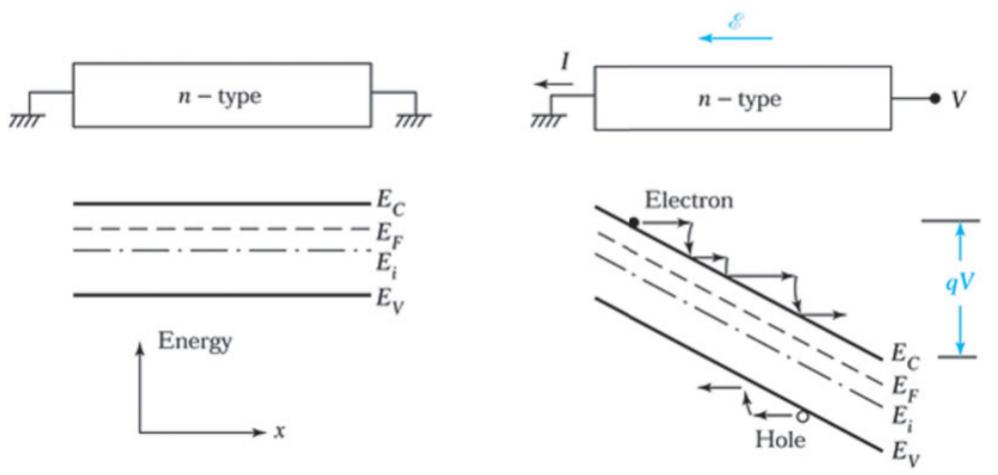
\includegraphics[width=12cm]{figures/ch01/bandbiasing.jpg}
\caption{Band structure under biasing} 
\label{fig:bandbiasing}
\end{figure}
Les électrons de la bande de conduction se déplacent vers le côté droit. L'énergie cinétique correspond à la distance par rapport au bord de bande (c'est-à-dire $E_C$ pour les électrons). Lorsqu'un électron subit une collision, il perd une partie ou la totalité de son énergie cinétique vers le réseau cristallin et retourne à sa position d'équilibre thermique. C'est l'origine du facteur d'atténuation $\alpha$ de la section précédente. Après que l'électron a perdu une partie ou la totalité de son énergie cinétique, il commencera à nouveau à se déplacer vers la droite et le même processus se répétera plusieurs fois. La conduction par les trous peut être visualisée de manière similaire mais dans la direction opposée.

\subsection{Courant de diffusion}
Un autre mécanisme de transport est la diffusion où les porteurs se déplacent d'un endroit à un autre en raison de la variation spatiale de la concentration de porteurs. Comme les porteurs se déplacent au hasard en raison de l'agitation thermique, plus de porteurs se déplaceront de la concentration de porteurs plus élevée vers celle de porteurs plus faible que dans l'autre sens, entraînant efficacement un mouvement net d'électrons de gauche à droite comme dans la figure \ref{fig:diffusion}. Ce courant est décrit par une équation de diffusion standard :
$$
J_n = q D_n \frac{dn}{dx}
$$
avec $D_p$ le coefficient de diffusion des trous. Une relation equivalente existe pour les trous:
$$
J_p = -q D_p \frac{dp}{dx}
$$
\begin{figure}[h!]
\centering
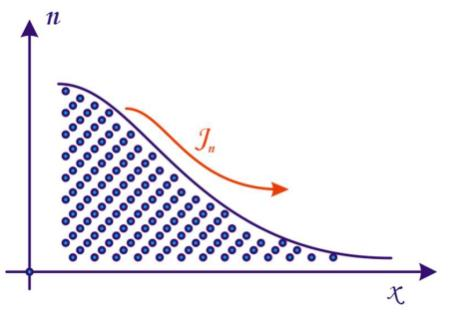
\includegraphics[width=8cm]{figures/ch01/diffusion.jpg}
\caption{Courant $J_n$ dû à la diffusion} 
\label{fig:diffusion}
\end{figure}
Cependant, ce déplacement de porteurs induira un champ électrique $\mathcal{E}$ et donc également un courant de dérive $J = q \mu_n n \mathcal{E}$. Après un certain temps, les deux courants seront égaux et opposés et un équilibre dynamique sera atteint :
$$
J_n = q \mu_n n \mathcal{E} +  q D_n \frac{dn}{dx} = 0
$$
En utilisant les équations de Boltzmann (\ref{eq:boltzamnn_eqns}), on peut déduire une relation entre $D_n$ et $\mu_n$ :
$$
D_n = \frac{kT}{q} \mu_n
$$
et
$$
D_p = \frac{kT}{q} \mu_p
$$
Ces relations sont connues sous le nom d'équations d'Einstein.
\section{Génération et Recombinaison}
\label{sec:generationrecombination}
En équilibre thermique, la relation $pn=n_i^2$ est valide. Il s'agit d'un équilibre dynamique : la génération thermique de paires électron-trou à un taux $G_{th}$ est contrebalancée par les électrons qui retombent de la bande de conduction à la bande de valence (c'est-à-dire un électron libre qui se combine avec un trou pour former une liaison covalente). Ce processus s'appelle la recombinaison.\\
Si des porteurs en excès sont introduits, nous ne sommes plus en équilibre et $pn>n_i^2$. La création de porteurs en excès est appelée \emph{injection de porteurs} et peut être réalisée par excitation optique ou en polarisant directement une jonction pn (voir le chapitre \ref{ch:pnjunction}). Le mécanisme qui rétablit l'équilibre est la recombinaison des porteurs minoritaires injectés avec les porteurs majoritaires présents dans le semi-conducteur. La génération et la recombinaison de porteurs thermiques et en excès sont représentées dans la figure \ref{fig:generationrecombination}.
\begin{figure}[h!]
\centering
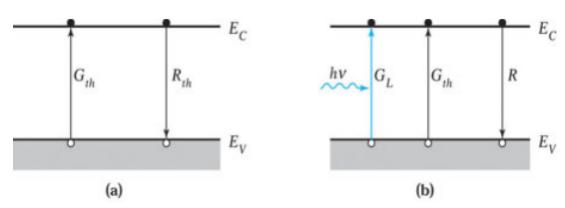
\includegraphics[width=12cm]{figures/ch01/recombination.jpg}
\caption{Generation and recombination under (a) equilibrium and (b) optical excitation} 
\label{fig:recombination}
\end{figure}
Nous supposons que les porteurs en excès conduisent à une recombinaison à une vitesse $R(n, p, T)$. À l'équilibre, $G_{th}(n_0, p_0, T) = R(n_0, p_0, T) = R_{th}$. Lorsque nous créons des porteurs en excès, nous pouvons écrire que $n = n_0 + \delta n$ et $p = p_0 + \delta p$, et nous supposerons que l'injection est faible par rapport aux conditions d'équilibre. Cela signifie que $\delta n \ll n_0$ et $\delta p \ll p_0$. Dans ces conditions, nous pouvons approximer la vitesse de recombinaison par les termes du premier ordre:
\begin{equation} 
\begin{split}
R(n, p, T) &= R(n_0, p_0, T) + (n-n_0) \frac{\partial R}{\partial n} + (p-p_0) \frac{\partial R}{\partial p} \\
           &= G_{th} +  \frac{(n-n_0)}{\tau_n} + \frac{(p-p_0)}{\tau_p} 
\end{split}
\end{equation} 
Dans un matériau de type n, le taux de recombinaison est déterminé par les trous en excès - car les trous sont beaucoup plus susceptibles de trouver un candidat pour la recombinaison (c'est-à-dire un électron) - que par les électrons en excès. Le taux auquel les porteurs recombinent est donc déterminé par le nombre de porteurs minoritaires :
\begin{itemize}
	\item En type n : $R - G_{th} = \frac{(p-p_0)}{\tau_p}$
	\item En type p : $R - G_{th} = \frac{(n-n_0)}{\tau_n}$
\end{itemize}
La durée de vie des porteurs minoritaires en excès $\tau_p$ et $\tau_n$ est beaucoup plus grande que le temps de relaxation $\tau_e$.
\section{Les équations de continuité}
Le changement de densité de porteurs dans un volume $V$ à l'intérieur d'un semi-conducteur peut être dû à trois causes :
\begin{enumerate}
	\item génération de porteurs,
	\item recombinaison,
	\item flux de porteurs entrant ou sortant du volume à travers la surface environnante $S$
\end{enumerate}
Supposons que nous voulons étudier le changement de la densité d'électrons dans un matériau de type p. Nous pouvons écrire:
\begin{equation} 
	\begin{split}
		-q \iiint_V \frac{\partial n}{\partial t} \; dV &= -q \iiint_V (G-R) \; dV - \varoiint_S \vec{J_n} \vec{n} \; dS \\
		 &= -q \iiint_V (G-R) \; dV - \iiint_V \nabla \vec{J_n}  \; dV \\
	\end{split}
\end{equation} 
où nous avons utilisé le théorème de la divergence. Comme cela est valable pour n'importe quel volume, les termes dans les intégrales doivent être égaux:
\begin{equation} 
	\begin{split}
		-q \frac{\partial n}{\partial t} &= -q (G-R) - \nabla \vec{J_n}\\
										 &= -q (G_{th} + g - R) - \nabla \vec{J_n}\\
	\Rightarrow	\frac{\partial n}{\partial t}	 &= \Big(\frac{n-n_0}{\tau_n}\Big) + \frac{1}{q}\nabla \vec{J_n} + g\\
	\end{split}
\end{equation}
où nous remplaçons $G_{th} - R$ par $\frac{(n-n_0)}{\tau_n}$ puisque nous sommes dans un matériau de type p. En une dimension, cela devient :
\begin{equation} 
	\begin{split}
		\frac{\partial n}{\partial t}	 &= \Big(\frac{n-n_0}{\tau_n}\Big) + \frac{1}{q} \frac{\partial J_n}{\partial x} + g\\
	\end{split}
\label{eq:continuity1}
\end{equation}
où $J_n$ a en général une contribution de dérive et de diffusion : $J_n = q \mu_n n \mathcal{E} + q D_n \frac{dn}{dx}$. En substituant cela dans \ref{eq:continuity1} - avec à la fois $n$ et $\mathcal{E}$ dépendant de $x$ - nous obtenons:
\begin{equation} 
	\begin{split}
		\frac{\partial n}{\partial t}	 &= \Big(\frac{n-n_0}{\tau_n}\Big) - n \mu_n \frac{\partial \mathcal{E}}{\partial x} + \mu_n \mathcal{E} \frac{\partial n}{\partial x} + D_n \frac{\partial^2 n}{\partial x^2} + g\\
	\end{split}
	\label{eq:continuity}
\end{equation}

Cette équation est appelée l'\emph{équation de continuité} pour les porteurs de type n dans un matériau de type p. Des expressions similaires peuvent être trouvées pour les autres cas.

%\begin{equation} 
%\begin{split}
%\frac{\partial n_p}{\partial t} &= n_p \mu_n \frac{\partial \mathcal{E}}{\partial x} + \mu_n \mathcal{E} \frac{\partial n_p}{\partial x} + D_n \frac{\partial^2 n_p}{\partial x^2} + G_{th} - \frac{n_p-n_{p0}}{\tau_n}\\
%\frac{\partial p_n}{\partial t} &= p_n \mu_p \frac{\partial \mathcal{E}}{\partial x} + \mu_p \mathcal{E} \frac{\partial p_n}{\partial x} + D_p \frac{\partial^2 p_n}{\partial x^2} + G_{th} - \frac{p_n-p_{n0}}{\tau_p}\\
%\end{split}
%\label{eq:continuity}
%\end{equation} 